\section{Generalization across models}\label{sec:multimodel}

The decomposition so far is on a single model. We rerun the entire protocol --- per-model operating-point selection under the coherence gate, both vector families, all projections and controls --- on two further instruction-tuned models from different families: Mistral-7B-Instruct-v0.3 and Qwen2.5-7B-Instruct. The RMSNorm-corrected construction transfers unchanged; only the per-model operating points differ. Table~\ref{tab:multimodel} and Figure~\ref{fig:multimodel} report the result, and it separates cleanly into a part that replicates and a part that does not.

\begin{table}[t]
\centering
\small
\begin{tabular}{llccc}
\toprule
model & family & $\Delta$MC2 [95\% CI] & $\rho$ (al-64) [95\% CI] & aligned$-$random [95\% CI] \\
\midrule
Llama-3-8B-Instruct & CAA & $-0.035$ {\scriptsize $[-0.071, +0.001]$} & $1.20$ {\scriptsize $[0.26, 3.35]$} & $+0.22$ {\scriptsize $[-0.98, +1.92]$} \\
 & mass-mean & $+0.073$ {\scriptsize $[+0.038, +0.107]$} & $0.95$ {\scriptsize $[0.79, 1.13]$} & $-0.07$ {\scriptsize $[-0.23, +0.11]$} \\
\midrule
Mistral-7B-Instruct-v0.3 & CAA & $-0.059$ {\scriptsize $[-0.096, -0.023]$} & $0.81$ {\scriptsize $[0.55, 1.02]$} & $-0.14$ {\scriptsize $[-0.36, +0.10]$} \\
 & mass-mean & $+0.069$ {\scriptsize $[+0.035, +0.102]$} & $0.74$ {\scriptsize $[0.48, 0.89]$} & $-0.24$ {\scriptsize $[-0.51, -0.08]$} \\
\midrule
Qwen2.5-7B-Instruct & CAA & $+0.008$ {\scriptsize $[-0.017, +0.033]$} & $1.73$ {\scriptsize $[-6.45, 8.10]$} & $+0.53$ {\scriptsize $[-5.57, +5.48]$} \\
 & mass-mean & $+0.005$ {\scriptsize $[-0.025, +0.034]$} & $0.67$ {\scriptsize $[-3.61, 5.60]$} & $+0.04$ {\scriptsize $[-4.69, +4.72]$} \\
\bottomrule
\end{tabular}

\caption{The headline statistics across three model families, each at its own coherence-gated operating point. $\Delta$MC2 is the family's test-set steering effect; $\rho$ is the fraction surviving aligned-64 excision; ``aligned$-$random'' is the paired contrast against random subspaces of equal rank. $\rho$ is interpretable only where $\Delta$MC2 is bounded away from zero (mass-mean on Llama-3 and Mistral); elsewhere it is greyed by the same rule used in the main text.}
\label{tab:multimodel}
\end{table}

\begin{figure}[t]
\centering
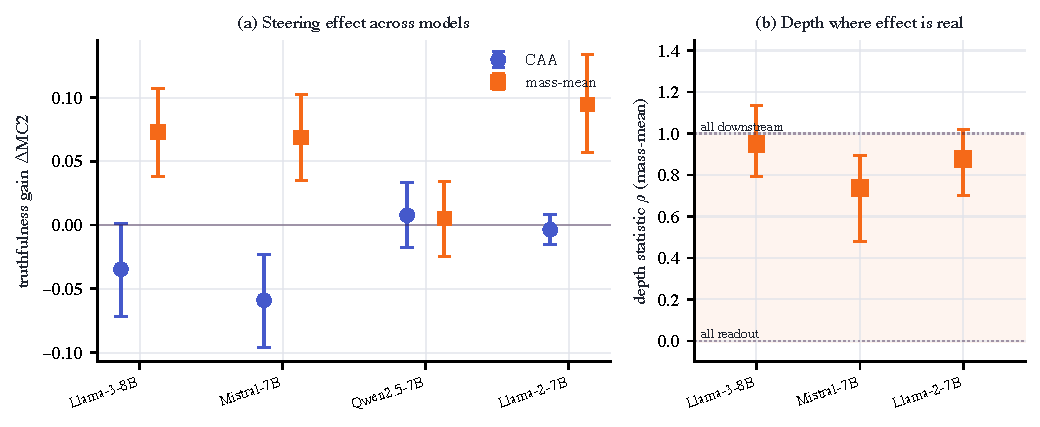
\includegraphics[width=0.82\textwidth]{../figures/multimodel.pdf}
\caption{Depth statistic $\rho$ (aligned-64, MC2) for both families on all three models, with 95\% intervals. CAA (blue) has no significant denominator on any model, so its $\rho$ is not interpretable; mass-mean (green) has a real effect on Llama-3 and Mistral, where $\rho$ is well above zero.}
\label{fig:multimodel}
\end{figure}

\paragraph{The CAA failure is universal.}
On no model does the contrastive vector improve truthfulness at a coherent operating point. Its test-set $\Delta$MC2 is \LlamaDecDelta{} on Llama-3, \MistralDecDelta{} \MistralDecDeltaCI{} on Mistral (significantly \emph{negative}), and \QwenDecDelta{} \QwenDecDeltaCI{} on Qwen (indistinguishable from zero). The vocabulary-level construction does not work anywhere, and on no model is its $\rho$ interpretable, because its denominator is never bounded away from zero. The complementary half of the dissociation is therefore the robust one.

\paragraph{The mass-mean effect is model-dependent.}
The mass-mean construction improves truthfulness on Llama-3 (\LlamaMmDelta{} \LlamaMmDeltaCI) and Mistral (\MistralMmDelta{} \MistralMmDeltaCI), both significant, but \emph{not} on Qwen (\QwenMmDelta{} \QwenMmDeltaCI, indistinguishable from zero). Where the effect is absent, the depth question is moot: Qwen's $\rho$ has the same uninterpretable-denominator status as CAA everywhere. We report this plainly --- the existence of a steering effect from this construction does not itself generalize across model families.

\paragraph{Where the effect exists, it is predominantly downstream.}
On both models with a real mass-mean effect, the majority survives certified excision of the direct readout: $\rho = \LlamaMmRho$ \LlamaMmRhoCI{} on Llama-3 and $\rho = \MistralMmRho$ \MistralMmRhoCI{} on Mistral. Neither is close to the $\rho \approx 0$ that pure vocabulary suppression predicts. The two models differ in one informative way. On Llama-3 the readout-aligned subspace is no more important than a random one of equal rank (aligned$-$random $= \LlamaMmAmr$ \LlamaMmAmrCI, not significant): the effect is essentially all downstream. On Mistral the aligned excision costs significantly more than random (aligned$-$random $= \MistralMmAmr$ \MistralMmAmrCI), so a minority of the Mistral effect --- roughly a quarter --- does run through the direct readout, with the remaining three quarters downstream. The picture across models is consistent: the contrastive construction is vocabulary-level and ineffective; the mass-mean effect, where it exists, is carried predominantly (Mistral) to almost entirely (Llama-3) by downstream computation rather than by the direct vocabulary readout.
